\documentclass{paper}
\usepackage{tikz}
\newcommand{\drawEdge}[5]{
  \draw[->] (#1) to[#5] node[midway, above] (#3Above) {$#4$} (#2);
  \draw[->] (#1) to[#5] node[midway, below] (#3Below) {} (#2);
}
\begin{document}

\section*{Intension}
In order to understand the notation fo whiskering $\mu H, H\mu$, we need to understand the composition of natural transformations.

\section*{Composition of Natural Transformations}
% I choose to neglect natural conditions since they are not relevant to the composition of natural transformations.

Entities we used in the diagram:

\begin{itemize}
  \item Categories: A,B,C
  \item Functors: $F,G,H,J,K,L$
  \item Natural Transformations: $\mu_1, \mu_2, \eta_1, \eta_2$
\end{itemize}


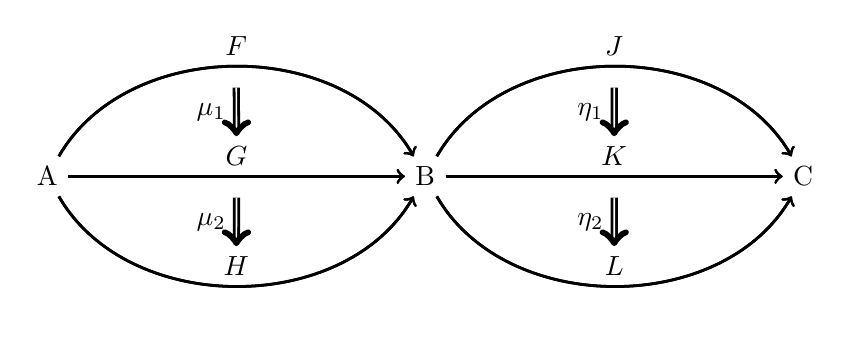
\begin{tikzpicture}[line width=1pt, scale=0.8]
  % Nodes
  \node (A) at (0,0) {A};
  \node (B) at (6,0) {B};
  \node (C) at (12,0) {C};
  \drawEdge{A}{B}{F}{F}{bend left=60}
  \drawEdge{A}{B}{G}{G}{bend right=0}
  \drawEdge{A}{B}{H}{H}{bend right=60}
  \draw[->, double] (FBelow) -- (GAbove) node[midway, left] {$\mu_1$};
  \draw[->, double] (GBelow) -- (HAbove) node[midway, left] {$\mu_2$};

  \drawEdge{B}{C}{J}{J}{bend left=60}
  \drawEdge{B}{C}{K}{K}{bend right=0}
  \drawEdge{B}{C}{L}{L}{bend right=60}
  \draw[->, double] (JBelow) -- (KAbove) node[midway, left] {$\eta_1$};
  \draw[->, double] (KBelow) -- (LAbove) node[midway, left] {$\eta_2$};
\end{tikzpicture}

\subsection*{Vertical Composition}
$\eta_1 \circ \mu_1 : F \Rightarrow H$.
Note that the composition is possible because the codomain of $\mu_1$ is the domain of $\eta_1$.

we also have $\eta_2 \circ \mu_2 : G \Rightarrow L$.

\subsection*{Horizontal Composition}

$\mu_2 \circ \mu_1 : J \circ F \Rightarrow K \circ G$.
Note that the composition is possible since: $\mathit{CoD_F} = \mathit{Do_J}$ and $\mathit{CoD_G} = \mathit{Do_K}$.

\pagebreak


\section*{Whiskering}
(To make things easier, I will use endo-functors $I, F$ on category $C$.)


$\mu F$ is an odd notation, since $\mu : I \Rightarrow F $ is natural transformation and $F$ is a functor.
It is called the right whiskering of $\mu$ with $F$.
It is the result of horizontally composing $\mu$ with $\mathit{id_F}$.
The left whiskering works similarly.

The process of whiskering is shown below:

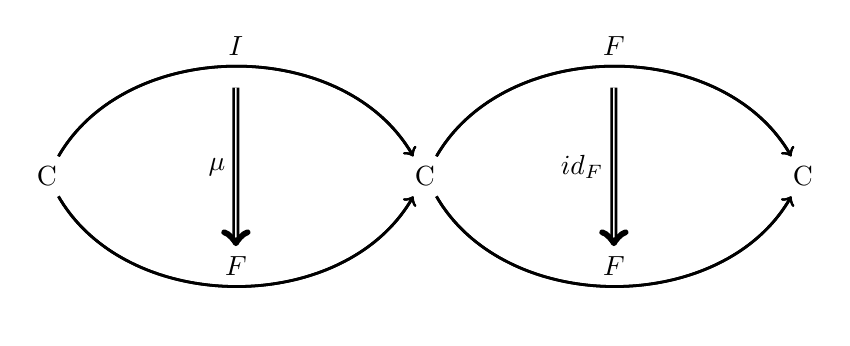
\begin{tikzpicture}[line width=1pt, scale=0.8]
  % Nodes
  \node (A) at (0,0) {C};
  \node (B) at (6,0) {C};
  \node (C) at (12,0) {C};
  \drawEdge{A}{B}{F}{I}{bend left=60}
  \drawEdge{A}{B}{G}{F}{bend right=60}
  \draw[->, double] (FBelow) -- (GAbove) node[midway, left] {$\mu$};

  \drawEdge{B}{C}{J}{F}{bend left=60}
  \drawEdge{B}{C}{K}{F}{bend right=60}
  \draw[->, double] (JBelow) -- (KAbove) node[midway, left] {$id_F$};
\end{tikzpicture}

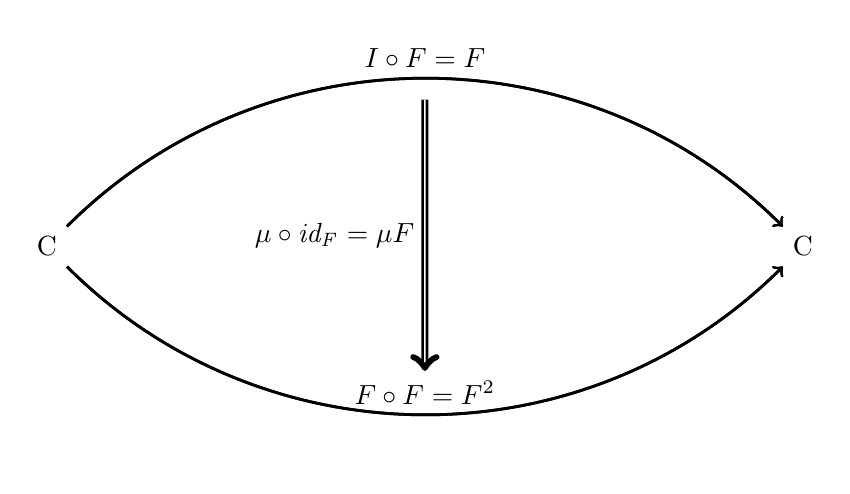
\begin{tikzpicture}[line width=1pt, scale=0.8]
  % Nodes
  \node (A) at (0,0) {C};
  \node (B) at (12,0) {C};
  \drawEdge{A}{B}{F}{I \circ F = F}{bend left=45}
  \drawEdge{A}{B}{G}{F \circ F = F^2}{bend right=45}
  \draw[->, double] (FBelow) -- (GAbove) node[midway, left] {$\mu \circ \mathit{id_F}= \mu F$};

\end{tikzpicture}
\end{document}
